\documentclass{beamer}
\mode<presentation>
{
	%\usetheme{CambridgeUS}
	\usetheme{Madrid}
	\usecolortheme{default}
	\usefonttheme{serif}
}
\usepackage[utf8]{inputenc}
\usepackage[russian]{babel}
\usepackage{cmap}
\usepackage{listings}
\usepackage{lmodern}
\usepackage{color}
\usepackage{minted}
\usepackage{graphicx}
\usepackage{tikz}
\usepackage{wrapfig}

\setbeamerfont{institute}{size=\normalsize}

\begin{document}
\title
[Форматирование текста программ на основе комбинаторов, сопоставления с образцом и синтаксических шаблонов]
{Форматирование текста программ на основе комбинаторов, сопоставления с образцом и синтаксических шаблонов}
\author
[Подкопаев Антон]{Подкопаев Антон, студент 445 группы, \texttt podkoav239@gmail.com}
\institute{СПбГУ \\
	\vspace{0.7cm}
	Научный руководитель: к.ф.-м.н. Булычев Д.Ю.
	\vspace{0.7cm}	
}
\date [15-04-13]{15 апреля 2013}

\begin{frame}[plain]
	\titlepage
\end{frame}

\begin{frame}{Контекст задачи}
	Языковые процессоры
	\vspace{1cm}
	\pause
	\begin{itemize}
		\item Компиляция
		\item Суперкомпиляция
		\item Интерпретация
		\item Статический анализ кода
		\item Декомпиляция
		\item Рефакторинг
		\item Реинжиниринг
	\end{itemize}
\end{frame}

\begin{frame}{План работы ЯП}
	\begin{itemize}
		\item Синтаксический анализ
		\item Преобразование
		\item Представление результата
		% Часто результат - программа на другом языке
		\pause
		\begin{itemize}
			\item \textcolor{red}{Код программы}
			\item ...
		\end{itemize}
	\end{itemize}
\end{frame}

\begin{frame}{ЯП}
	\begin{itemize}
		\item Компиляция
		\item Суперкомпиляция
		\item Интерпретация
		\item Статический анализ кода
		\item Декомпиляция
		\item Рефакторинг
		\item Реинжиниринг
	\end{itemize}
\end{frame}

\begin{frame}{ЯП}
	\begin{itemize}
		\item \textcolor{gray}{Компиляция}
		\item Суперкомпиляция
		\item \textcolor{gray}{Интерпретация}
		\item Статический анализ кода
		\item Декомпиляция
		\item Рефакторинг
		\item Реинжиниринг
	\end{itemize}
\end{frame}

\begin{frame}{Актуальность задачи}
	Почему нельзя просто взять и напечатать?
	\vspace{1cm}
	\pause
	\inputminted{c}{codes/wikiExUnfor.c}
\end{frame}

\begin{frame}[fragile]{Естественное описание}
	\begin{block}{}
		\inputminted{pascal}{codes/if1.pas}
	\end{block}
	\begin{block}{}
		\inputminted{pascal}{codes/if2.pas}
	\end{block}
	\begin{block}{}
		\inputminted{pascal}{codes/if3.pas}
	\end{block}
\end{frame}

\begin{frame}{Существующие решения}
	Комбинаторы
	\vspace{0.7cm}	
	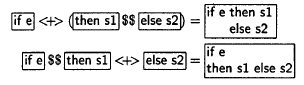
\includegraphics[width = 1\linewidth]{images/a1.png}
	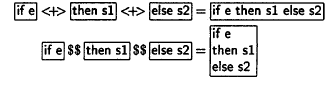
\includegraphics[width = 1\linewidth]{images/a2.png}
	\vspace{0.7cm}
	Построение документов с помощью некоторого набора комбинаторов
\end{frame}

\begin{frame}{Пример комбинаторного принтера}
	\inputminted{haskell}{codes/lHughesPrinter.hs}
\end{frame}

\begin{frame}{Решение}
	Шаблоны
	\begin{block}{}
		\inputminted{pascal}{codes/l_write.t}
	\end{block}
\end{frame}

% \begin{frame}{Необходимые части}
% 	\begin{itemize}
% 		\item Расширяемый парсер
% 		\ite
% 	\end{itemize}
% \end{frame}

\begin{frame}{Этапы работы}
	\begin{itemize}
		\item Получение расширенным парсером языка образцы
		\item Составление документа по дереву
	\end{itemize}
\end{frame}

\begin{frame}{Язык L}
	Небольшой Pascal-like язык
	\vspace{1cm}
	\begin{block}{}
		\inputminted{c}{codes/pow.l}
	\end{block}
\end{frame}

\begin{frame}{Пример шаблонов}
	\begin{block}{}
		\inputminted{pascal}{codes/l_while.t}
	\end{block}
\end{frame}

\begin{frame}{Результат}
	\begin{itemize}
		\item Доказательство состоятельности подхода
		\item Реализация подхода для языка L
	\end{itemize}
\end{frame}

\end{document}

